\begin{figure*}[t]
\centering
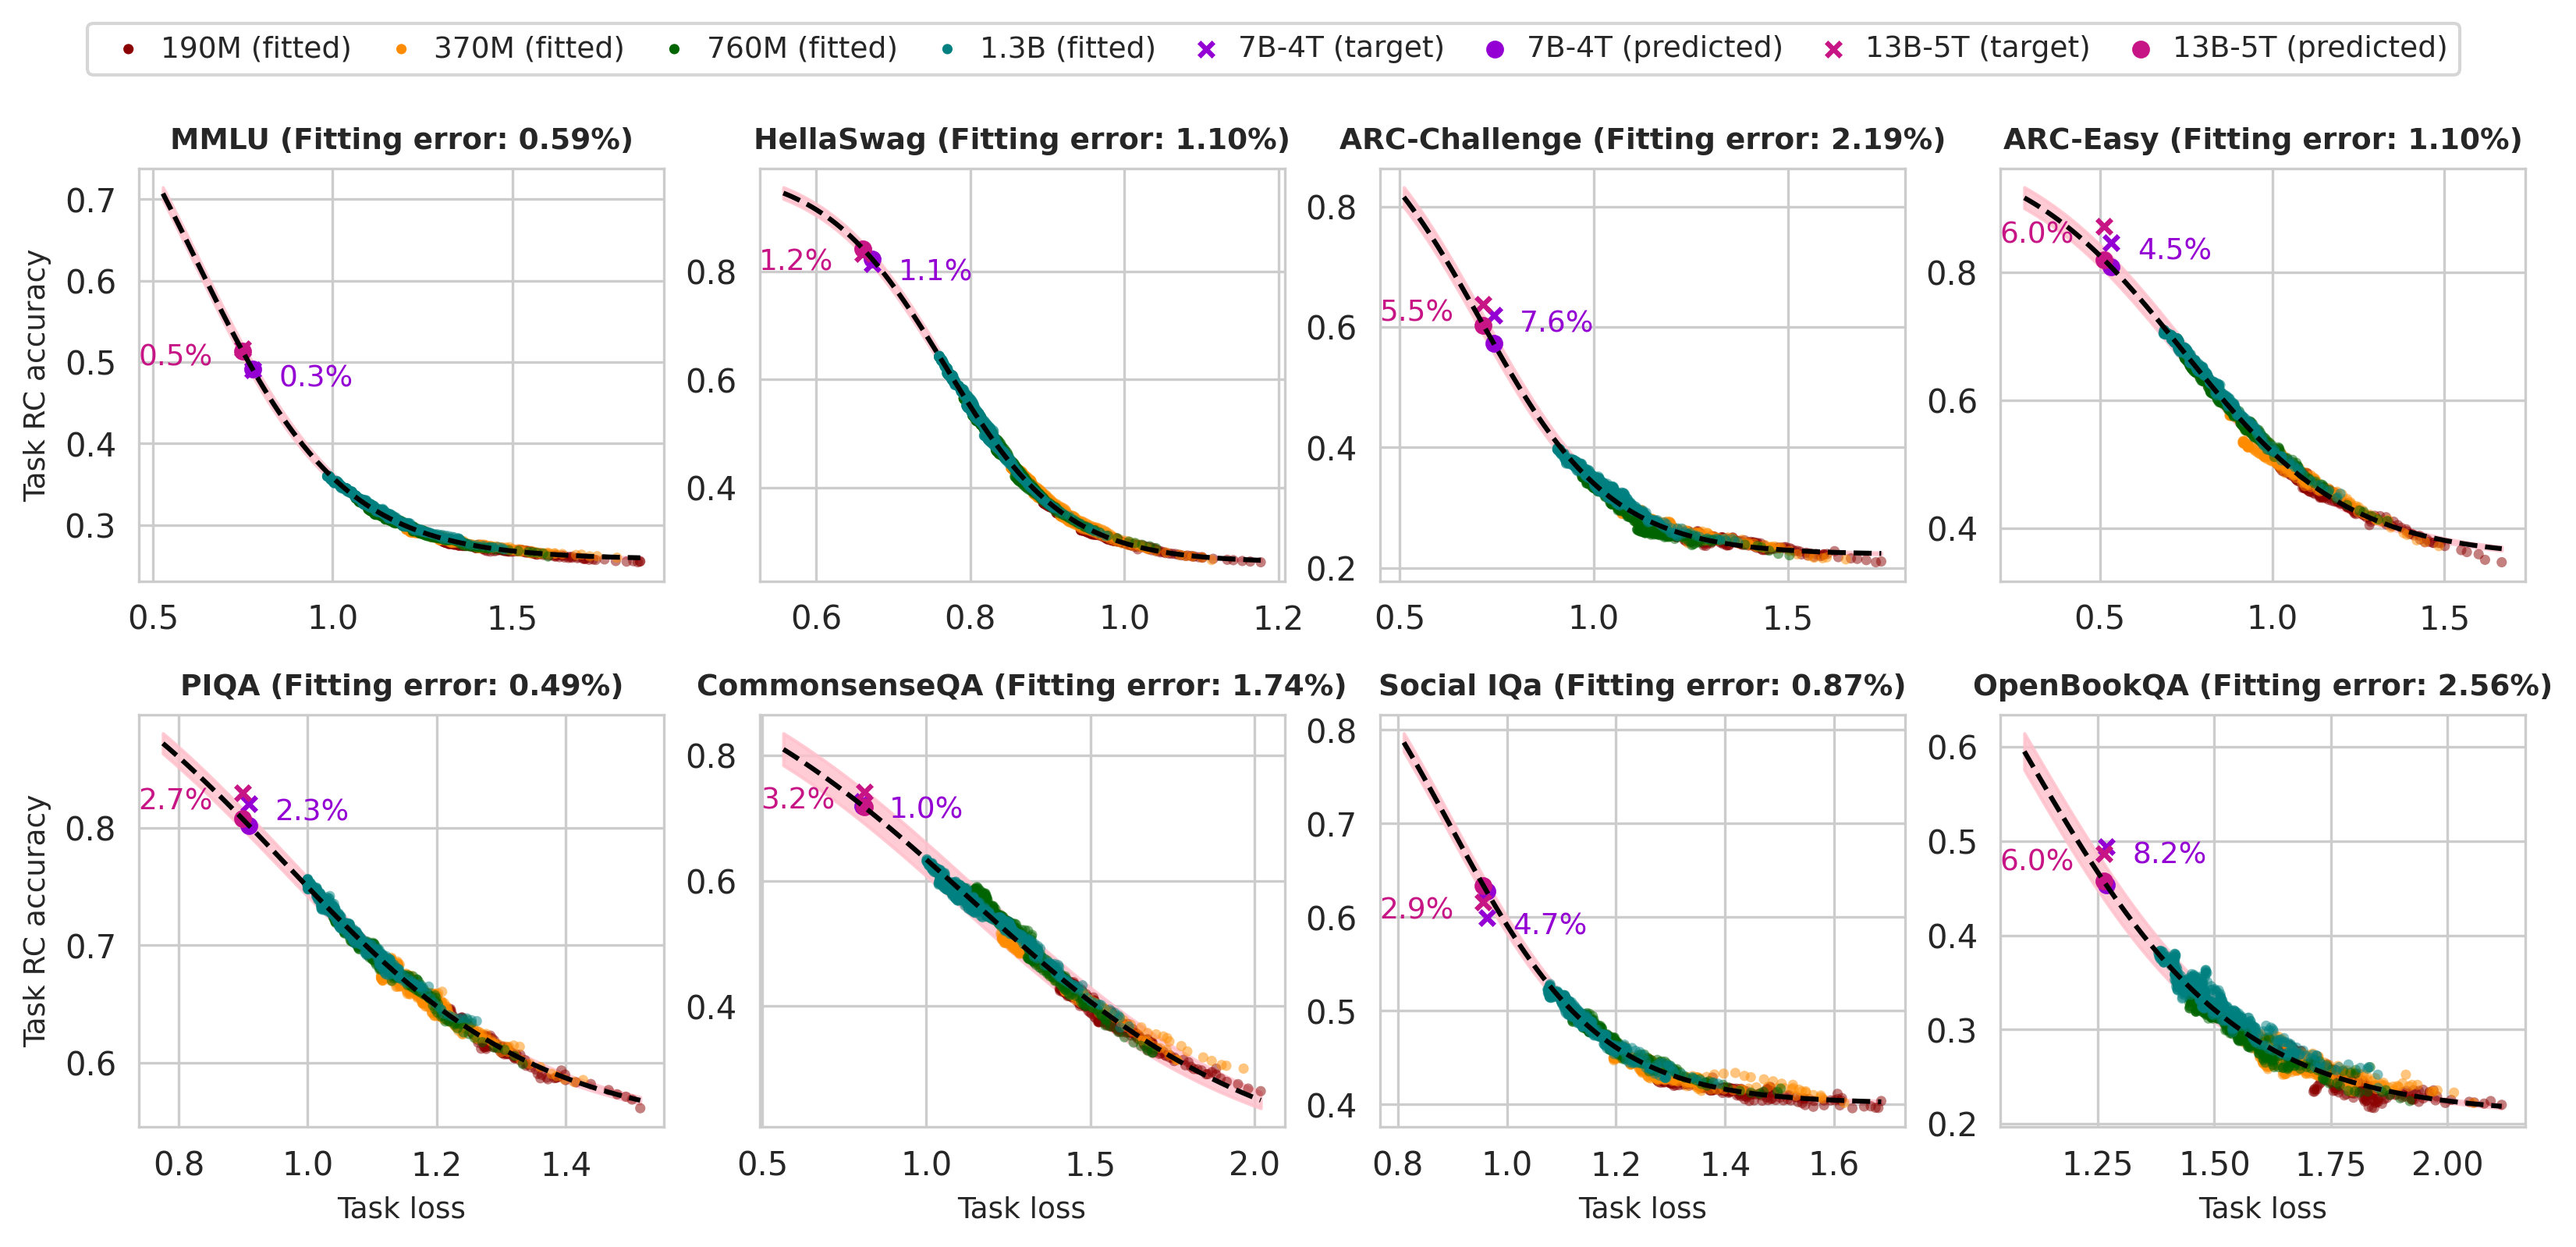
\includegraphics[width=\linewidth]{images/step2_main.png}
\vspace{-16pt}
\caption{
    Task RC accuracy vs task loss, with fitting on the sigmoid function in \autoref{eqn:sigmoid}.
    The prediction error is next to the target model point.
    %For each task, the data points collected from ladder models lie on a shared sigmoidal curve, and the fitted function makes rather reliable predictions for the target models. 
    The shaded area represents the prediction intervals for the fitted function.
    %See \autoref{tab:fitted_params} for the parameters of the fitted functions.
}
\label{fig:step2}
\vspace{-8pt}
\end{figure*}